\documentclass{article}
\usepackage{graphicx, mathtools, amsmath, amssymb, float}
\graphicspath{{Images/}}

\newcommand{\say}[1]{``#1"}


\setlength{\oddsidemargin}{0in}
\setlength{\textwidth}{6.5in}
\setlength{\topmargin}{-.55in}
\setlength{\textheight}{9in}
\pagestyle{empty}


\title{Homework 1}
\author{Michael Nameika}
\date{August 2023}

\begin{document}

\maketitle

\section*{1.1 Problems}
\begin{itemize}
    \item[\textbf{6}.] Show that $d$ in \textbf{1.1-6} satisfies the triangle inequality.
    \newline\newline
    \textit{Proof}: Let $X$ be the set of all bounded sequences and define $d: X \times X \to \mathbb{R}$ by
    \[d(x,y) = \sup_{i \in \mathbb{N}}|x_i - y_i|\]
    where $x_i$, $y_i$ are the $i^{\text{th}}$ elements of $x$, $y \in X$, respectively. 
    \newline

    Let $x,y,z \in X$. Then for any $i$, using the triangle inequality for $|\cdot|$, we have
    \begin{align*}
        |x_i - y_i| &= |x_i - z_i + z_i - y_i|\\
        &\leq |x_i - z_i| + |z_i - y_i|.
    \end{align*}
    Notice by definition of supremum,
    \begin{align*}
        |x_i - z_i| &\leq \sup_{i\in \mathbb{N}} |x_i - z_i|\\
        |z_i - y_i| &\leq \sup_{i\in \mathbb{N}} |z_i - y_i|.
    \end{align*}
    So then
    \begin{align*}
        |x_i - y_i| &\leq \sup_{i\in \mathbb{N}} |x_i - z_i| + \sup_{i\in \mathbb{N}} |z_i - y_i|\\
        &= d(x,z) + d(z,y)
    \end{align*}
    then $|x_i - y_i|$ is bounded above by $d(x,z) + d(z,y)$ for all $i$, hence
    \begin{align*}
        \sup_{i\in \mathbb{N}}|x_i - y_i| &\leq d(x,z) + d(z,y)\\
        d(x,y) &\leq d(x,z) + d(z,y).
    \end{align*}
    Hence, $d$ satisfies the triangle inequality.

    
    \item[\textbf{12}.] \textbf{(Triangle inequality)} The triangle inequality has several usefull consequences. For instance, using (1), show that 
    \[|d(x,y) - d(z,w)| \leq d(x,z) + d(y,w)\]
    \newline\newline
    \textit{Proof}: Let $(X,d)$ be a metric space and $x,y,z,w \in X$. By the triangle inequality, we have 
    \[d(x,y) \leq d(x,z) + d(z,w) + d(w,y)\]
    so that
    \begin{align*}
        |d(x,y) - d(z,w)| &= |d(x,z) + d(z,w) + d(w,y) - d(z,w)|\\
        &= |d(x,z) + d(y,w)|.
    \end{align*}
    Since $d(x,z) \geq 0$, $d(y,w) \geq 0$,
    \[|d(x,z) + d(w,y)| = d(x,z) + d(y,w)\]
    hence,
    \[|d(x,y) - d(z,w)| \leq d(x,z) + d(y,w).\]
\end{itemize}


\section*{1.2 Problems}
\begin{itemize}
    \item[\textbf{4}.] \textbf{(Space $l^p$)} Find a sequence which converges to 0, but is not in any space $l^p$, where $1 \leq p < + \infty$.
    \newline\newline
    Consider the sequence of real numbers $\{x_n\}$ defined by
    \[x_n = \frac{1}{\ln(n + 1)}.\]
    Notice since $\ln(n + 1) \to \infty$ as $n \to \infty$, so $\frac{1}{\ln(1 + n)} \to 0$ as $n \to \infty$. We will show that the series
    \[\sum_{n = 1}^{\infty} \frac{1}{|\ln(1 + n)|^p}\]
    diverges for all natural numbers $1 \leq p < +\infty$. Recall that
    \[\lim_{x \to \infty} \frac{x^n}{e^x} = 0\]
    for all natural numbers $n$. Hence, there exists some real number $x_0$ such that for all $x > x_0$,
    \[x^n < e^x.\]
    Take $x = \ln(y + 1) > x_0$ for $y + 1 > e^{x_0} = y_0$. Then by the above inequality, we have
    \[(\ln(y+1))^n < y + 1\]
    so
    \[\frac{1}{1 + y} < \frac{1}{(\ln(1 + y))^n}\]
    for all $y > y_0$. Then
    \[\sum_{k = \lceil y_0\rceil}^{\infty} \frac{1}{1 + y} < \sum_{k = \lceil y_0\rceil}^{\infty} \frac{1}{(\ln(1 + y))^n} < \sum_{k = 1}^{\infty} \frac{1}{(\ln(1 + y))^n}.\]
    Since $\sum_{k = \lceil k_0\rceil}^{\infty} \tfrac{1}{1 + y}$ diverges, by direct comparison, we have 
    \[\sum_{k = 1}^{\infty} \frac{1}{(\ln(1 + y))^n}\]
    diverges for all natural numbers $n$.

    


    
\end{itemize}

\section*{1.3 Problems}
\begin{itemize}
    \item[\textbf{8}.] Show that the closure $\overline{B(x_0;r)}$ of an open ball $B(x_0;r)$ in a metric space can differ from the closed ball $\overline{B}(x_0;r)$.
    \newline\newline
    \textit{Proof}: Consider the metric space $(\mathbb{Q}, d)$ where $\mathbb{Q}$ denotes the set of rational real numbers and $d(x,y) = |x - y|$. Let $x \in \mathbb{Q}$, $r > 0$ and consider the open ball of radius $r$ centered at $x$, 
    \[B_r(x) = \{y \in \mathbb{Q} \:|\: d(x,y) < r\}.\] 
    Then the closed ball of radius $r$ centered at $x$ is given by
    \[\overline{B}_r(x) = \{y \in \mathbb{Q} \:|\: d(x,y) \leq r\}.\]
    However, since the set of limit points of $\mathbb{Q}$ is all of $\mathbb{R}$, the closure of the open ball of radius $r$ is given by
    \[\overline{B_r(x)} = \{y \in \mathbb{R} \:|\: d(x,y) \leq r\}.\]
    Hence, $\overline{B_r(x)} \neq \overline{B}_r(x)$ since $\overline{B_r(x)}$ contains all irrational numbers in the interval $[x - r, x + r]$, but $\overline{B}_r(x)$ contains no irrational numbers in the interval $[x - r, x + r]$.
\end{itemize}



\section*{1.4 Problems}
\begin{itemize}
    \item[\textbf{6}.] If ($x_n$) and ($y_n$) are Cauchy sequences in a metric space ($X,d$), show that ($a_n$), where $a_n = d(x_n,y_n)$, converges. Give illustrative examples.
    \newline\newline
    \textit{Proof}: Let ($X,d$) be a metric space and $\{x_n\}$, $\{y_n\}$ be Cauchy sequences in ($X,d$). Define the sequence of real numbers $\{a_n\}$ by $a_n = d(x_n,y_n)$. Since $\mathbb{R}$ is a complete metric space, we will show that $\{a_n\}$ is a Cauchy sequence in $\mathbb{R}$ and is therefore convergent. 
    \newline
    Since $\{x_n\}$ and $\{y_n\}$ are Cauchy sequences in ($X,d$), there exist natural numbers $N_1,N_2$ such that whenever $n,m > N_1$, 
    \[d(x_n,x_m) < \frac{\epsilon}{2}\]
    and similarly, whenever $n,m > N_2$,
    \[d(y_n,y_m) < \frac{\epsilon}{2}.\]
    Take $N = \max\{N_1,N_2\}$ and $n,m > N$ and consider 
    \begin{align*}
        |a_n - a_m| &= |d(x_n,y_n) - d(x_m,y_m)|\\
        &\leq |d(x_n, x_m) + d(x_m, y_m) + d(y_m,y_n) - d(x_m,y_m)|\\
        &= |d(x_n,x_m) + d(y_n,y_m)|\\
        &= d(x_n,x_m) + d(y_n,y_m)\\
        &< \frac{\epsilon}{2} + \frac{\epsilon}{2}\\
        &= \epsilon.
    \end{align*}
    We then  have
    \[|a_n - a_m| < \epsilon.\]
    Hence, $\{a_n\}$ is a Cauchy sequence in $\mathbb{R}$.
    \newline

    As an example, consider the metric space $(\mathbb{R}, |\cdot|)$ and the sequences $\{x_n\}$ and $\{y_n\}$ defined by
    \begin{align*}
        x_n &= \frac{1}{n}\cos(n)\\
        y_n &= \log\left(1 + \frac{1}{n^{1/4}}\right)
    \end{align*}
    Clearly, these sequences converge in $\mathbb{R}$ and are therefore Cauchy by the completeness of $\mathbb{R}$. Define the sequence $\{a_n\}$ by
    \[a_n = |x_n - y_n| = \left|\frac{1}{n}\cos(n) - \log\left(1 + \frac{1}{n^{1/4}}\right)\right|\]
    From our work above, we have that $\{a_n\}$ converges in $\mathbb{R}$. An illustration of these sequences can be found in the following figure:
    
    \begin{figure}[H]
        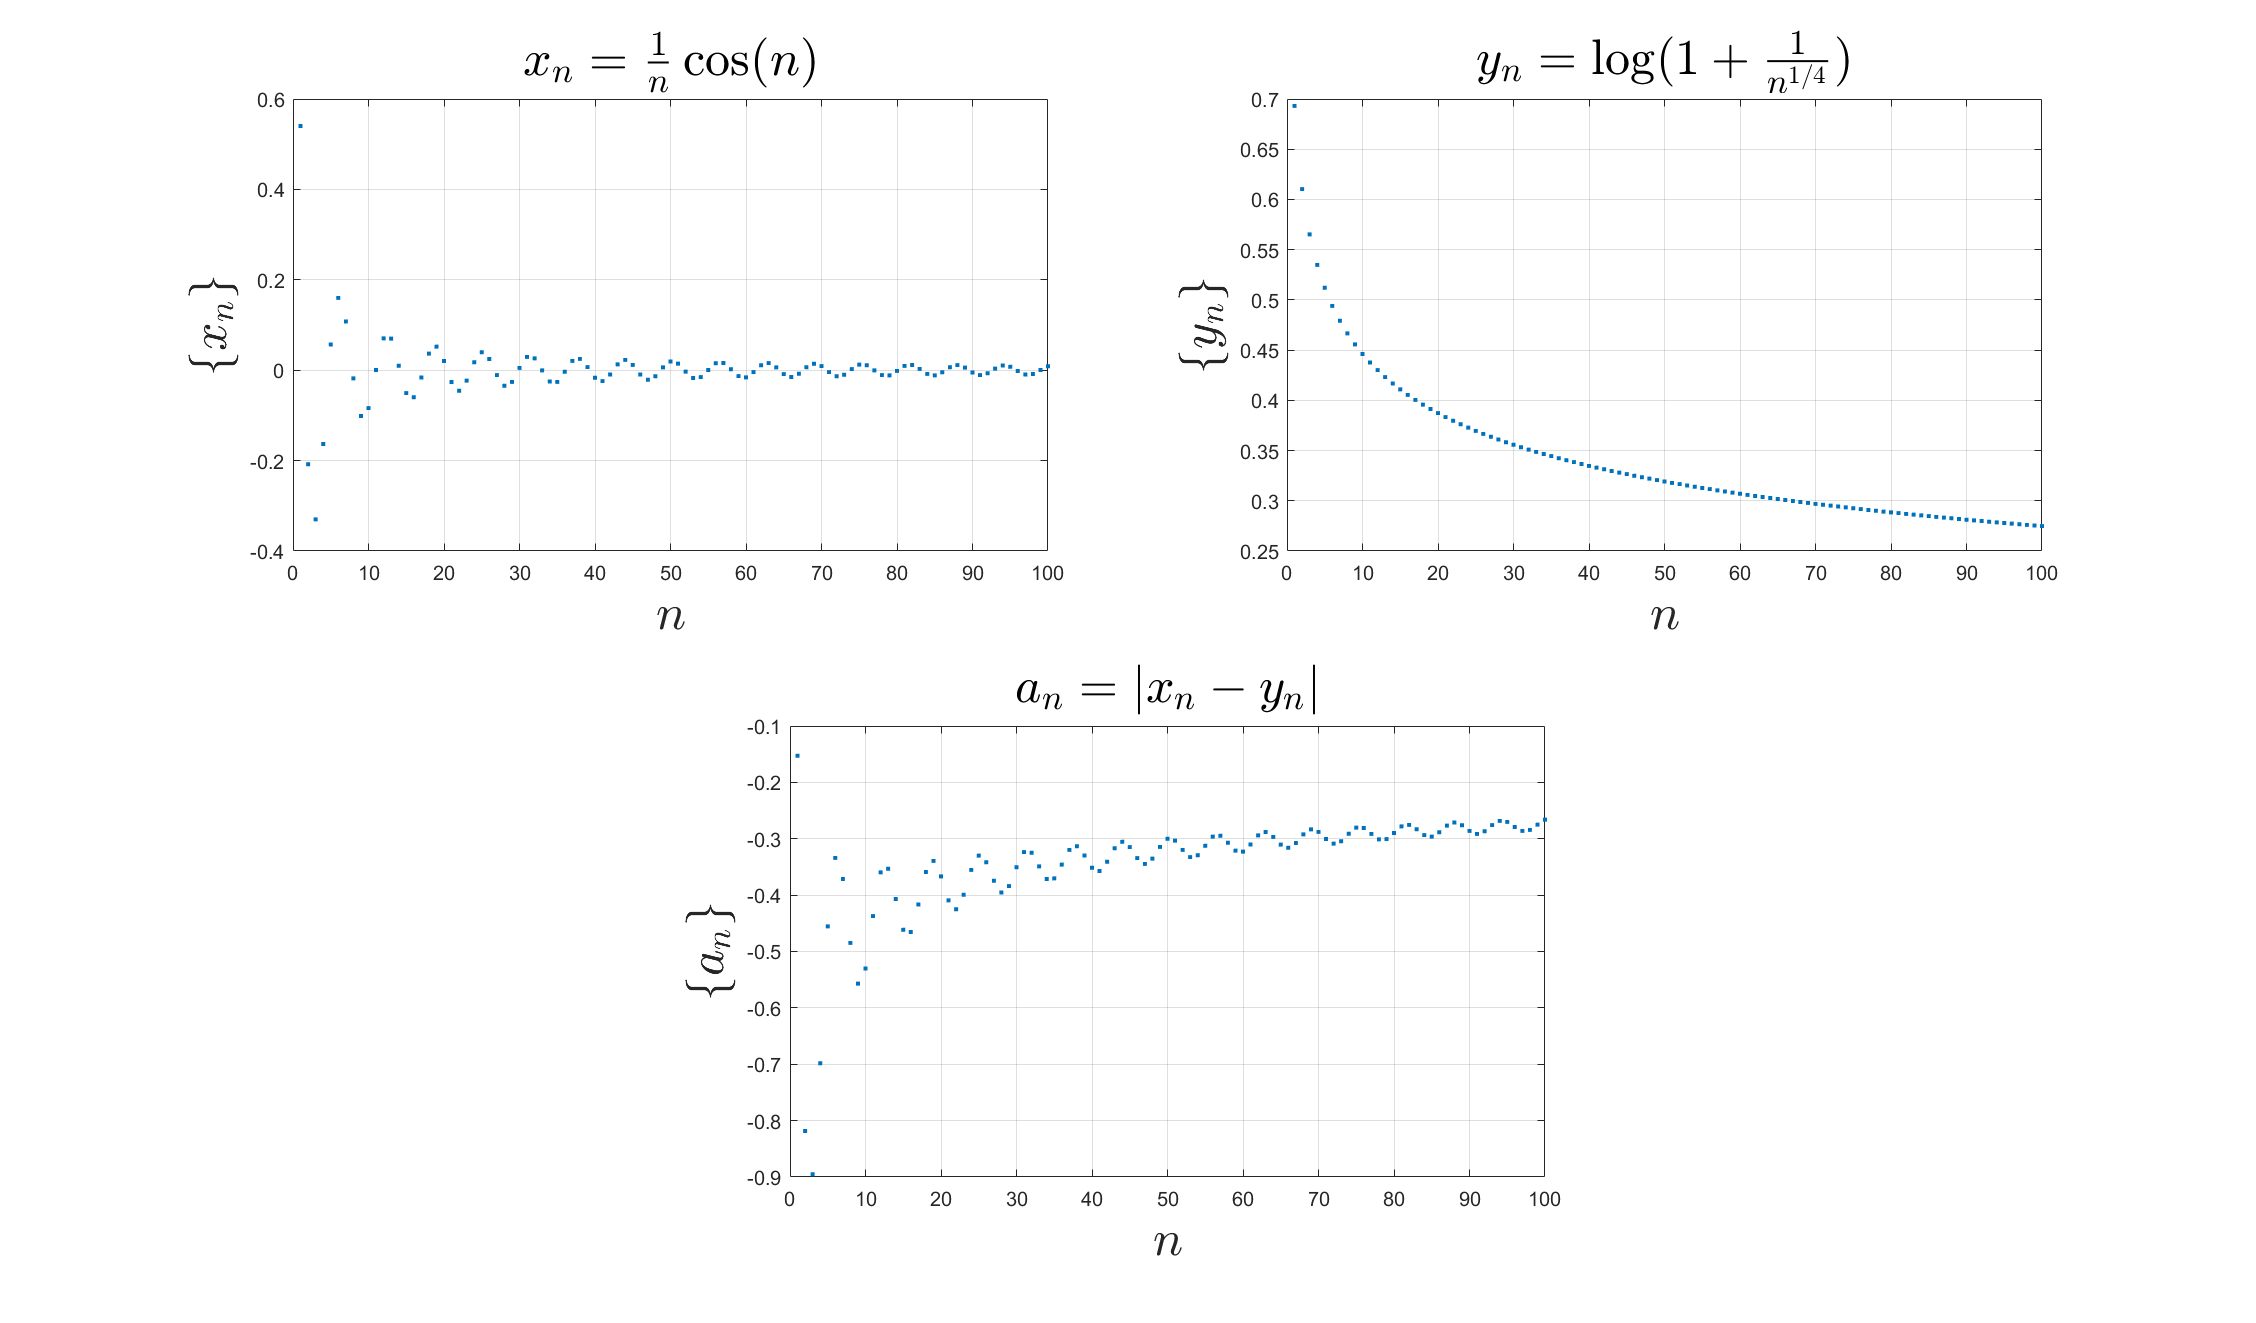
\includegraphics[scale = 0.3]{cauchySeqs.png}
        \centering
    \end{figure}
    For an example in an incomplete metric space, consider the space of polynomials on the interval $[-1,1]$ equipped with the sup metric, denote this space by $P[-1,1]$. Consider the Cauchy sequences $\{y_n\}$ and $\{z_n\}$ defined by
    \[y_n = \sum_{k=1}^n \frac{x^k}{k!}\]
    and
    \[z_n = \sum_{k=0}^n \frac{(-1)^k(\pi x)^{2k + 1}}{(2k + 1)!}\]
    Clearly, $y_n \to e^x$ and $z_n \to \sin(\pi x)$ in $C[-1,1]$, but $e^x$ and $\sin(\pi x)$  not in $P[-1,1]$. Hence, $P[-1,1]$ is an incomplete metric space. Now define the sequence $\{a_n\}$ of real numbers by $a_n = d(y_n,z_n) = \sup_{x \in [-1,1]} |y_n - z_n|$. By our work above, we know that $\{a_n\}$ converges. For a visualization, see the figure below.

    \begin{figure}[H]
        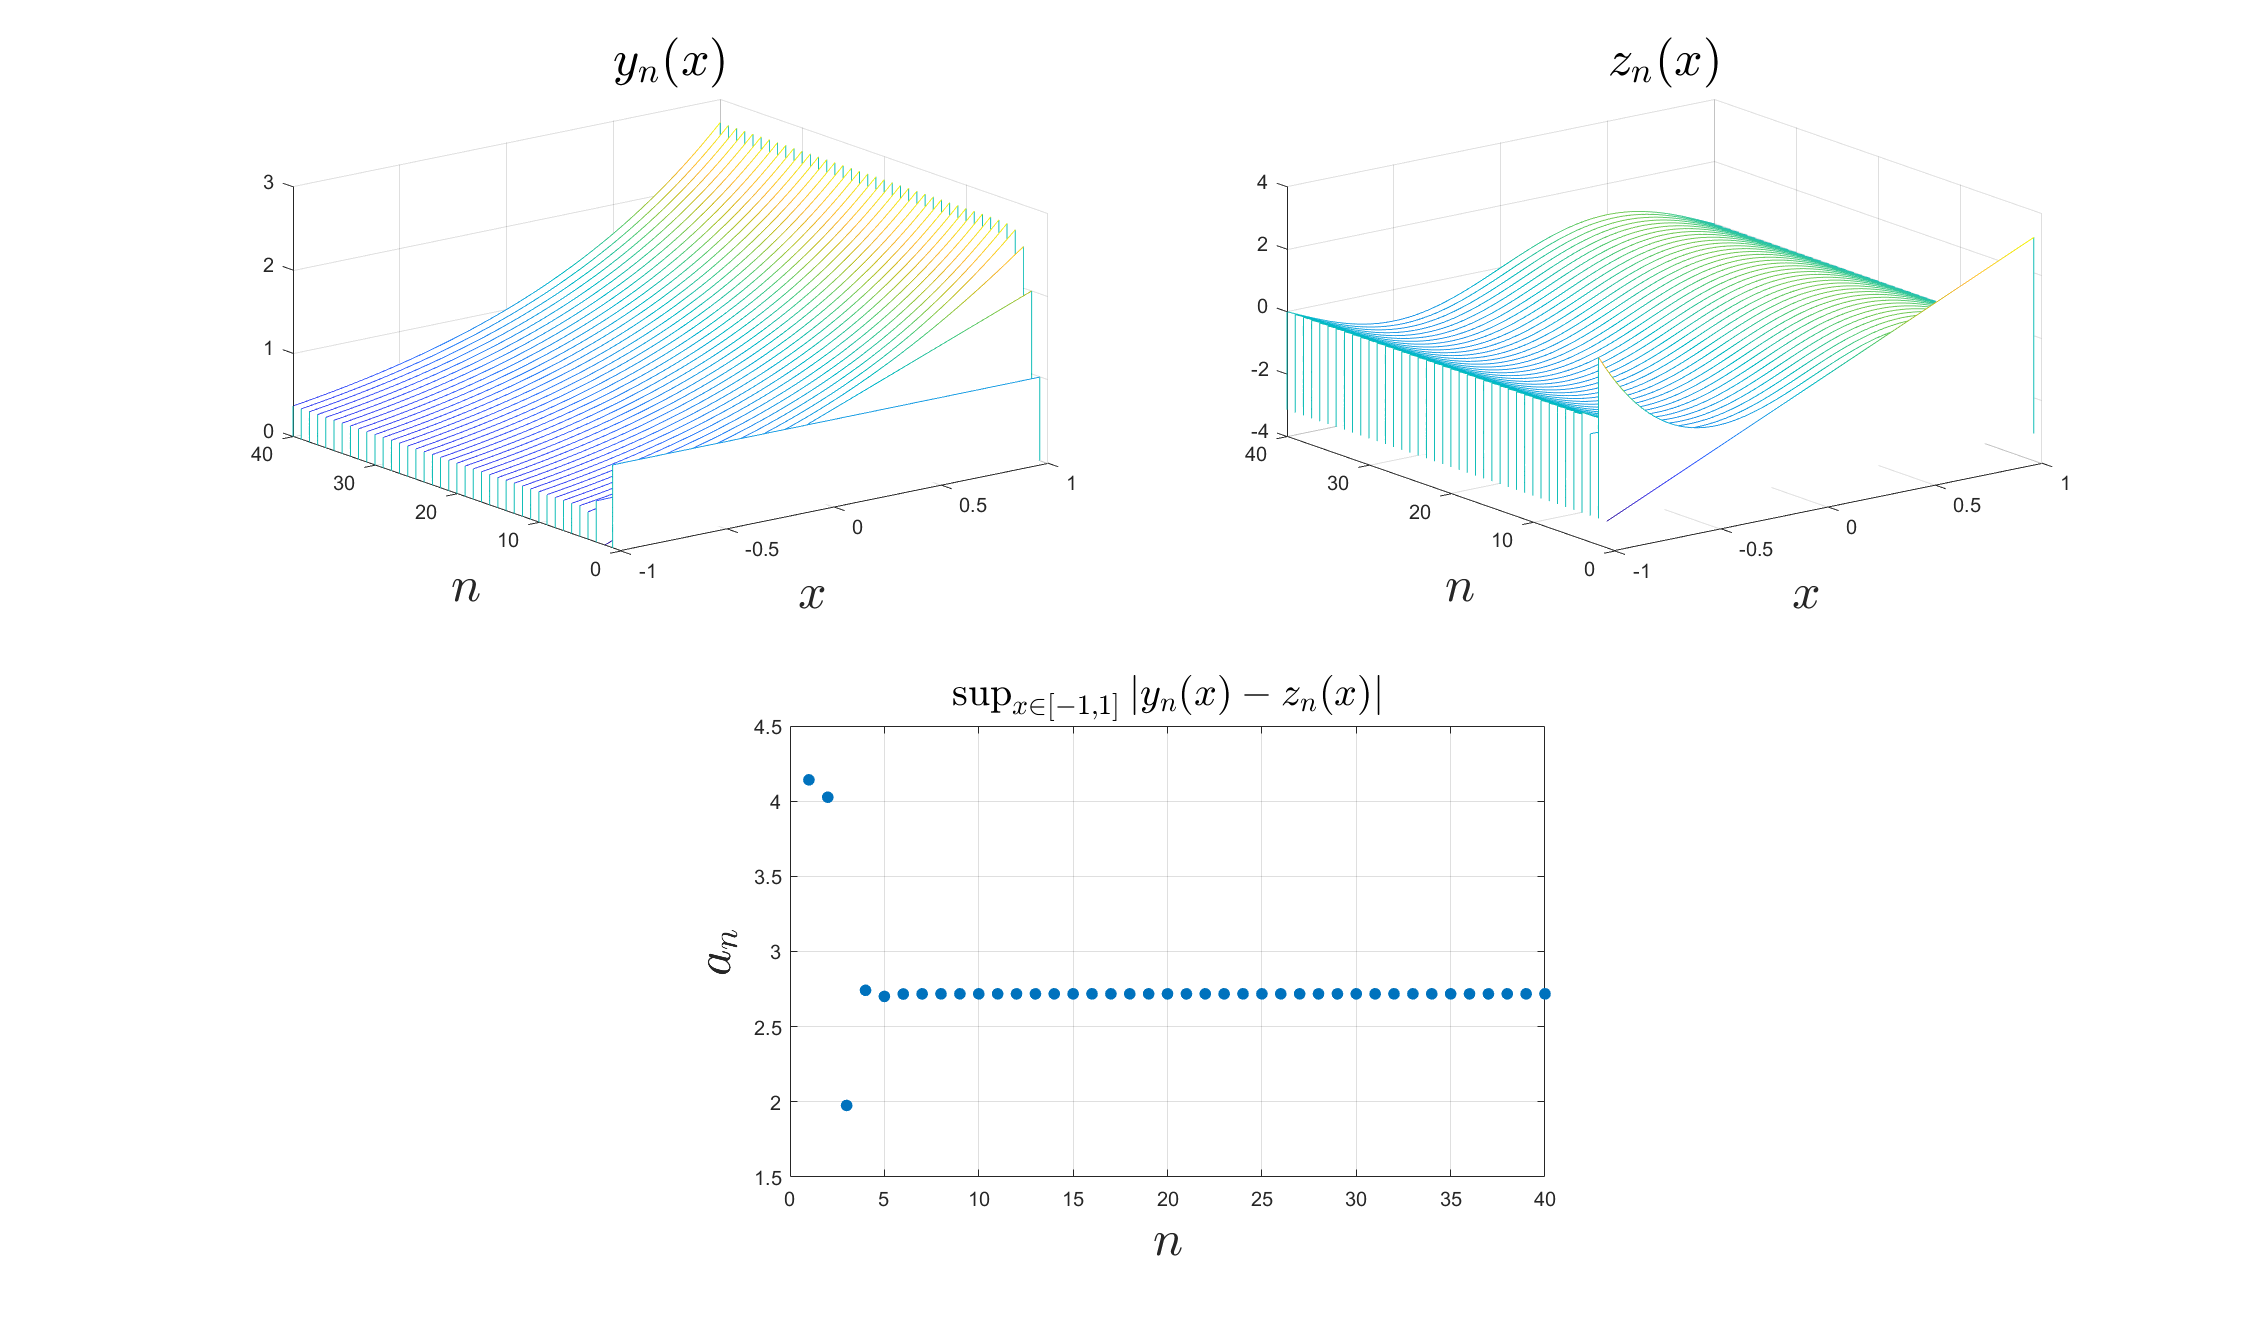
\includegraphics[scale = 0.3]{supExamp.png}
        \centering
        \caption{Plots for $y_n = \sum_{k=0}^n \tfrac{x^k}{k!}$, $z_n = \sum_{k=0}^n \tfrac{(-1)^k(\pi x)^{2k+1}}{(2k+1)!}$ and the sequence of their maximum difference, $a_n$, for various values of $n$.}
    \end{figure}
\end{itemize}




\end{document}
